\documentclass[epsfig]{article}
\usepackage{epsfig}
\usepackage{amsmath}
\usepackage{verbatim}
\usepackage{booktabs}
\usepackage{subfig}
\usepackage{graphicx}
\usepackage{multirow}
\usepackage{epsfig}
\usepackage{amsmath}
\usepackage{graphicx}
\usepackage{subfig}
\usepackage[english]{babel}
\usepackage{rotating}
\usepackage{multirow}
\usepackage[english]{babel}
\textwidth 6.7in
\oddsidemargin -0.1in
\textheight 8.50in
\topmargin -0.55in
\renewcommand{\textfraction}{0.25}
\renewcommand{\floatpagefraction}{0.7}
\begin{document}
\parindent=0pt
\author{Kentaro Hoffman}
\title{COMP/ELEC/STAT 502 HW 07}
\maketitle

  
 \section*{Problem 1}
 \subsection*{a)}
 \begin{table}[htbp] 
\center
\caption{Parameters for LVQ1}
  \label{tab:NP}
  %\scalebox{0.9}{ % You can scale the size of the table by changing this number
   \scalebox{1.0}{
   \begin{tabular}{p{6cm} p{.05cm} p{8cm}}
\toprule
  \multicolumn{3}{l}{\bf Network parameters} \\
\bottomrule \noalign{\smallskip}
  Topology & & 64 Prototypes in a 8x8 grid Covering the whole Dataspace, ie (1,1) to (9,9)  \\
\toprule
  \multicolumn{3}{l}{\bf Learning parameters} \\
\bottomrule \noalign{\smallskip}
  Initial weights & & drawn from (U[1, 9], U[1, 9]) \\
   Learning rates & & 0.02, 0.01, 0.005, 0.001\\
  Decay of the Learning Rate (Learning Steps)  && 30,000, 50,000, 120,000 , Never\\
  Number of Learning Steps  & & 150,000\\
  
  \\\toprule
 \multicolumn{3}{l}{\bf Input / output data, representation, scaling} \\
\bottomrule \noalign{\smallskip}
Training Data && 81 data points equally distributed along a grid from (1,1) to (9,9).\\
Scaling of Training Data && None\\
Testing Data && 900 data points equally distributed along a grid from (1,1) to (9,9).\\
Scaling of Testing Data && None\\
Monitering Frequency && 10,000 \\
%  %\# learn steps performed & & 180,365 (error threshold reached)\\

 \bottomrule \noalign{\smallskip}
   \end{tabular}
   } 
\end{table}
\textbf{Decay Of the Learning Rate}\\
The learning rate was decayed using a step funtion. After a certain number (such as 30,000) of learning steps, the learning rate would be decreased from the previous value (0.02) to the new value (0.01).
\newpage
\section*{Results}
\begin{center}
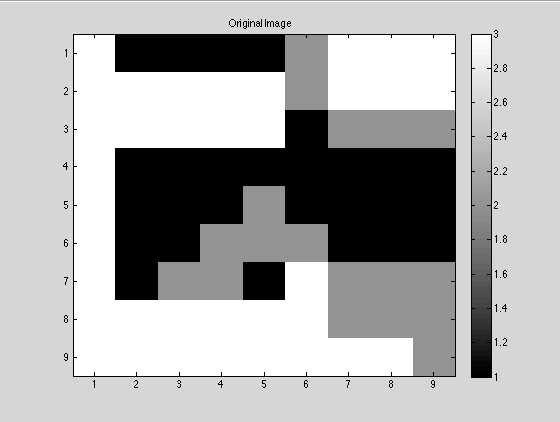
\includegraphics[scale=0.42]{pic1}
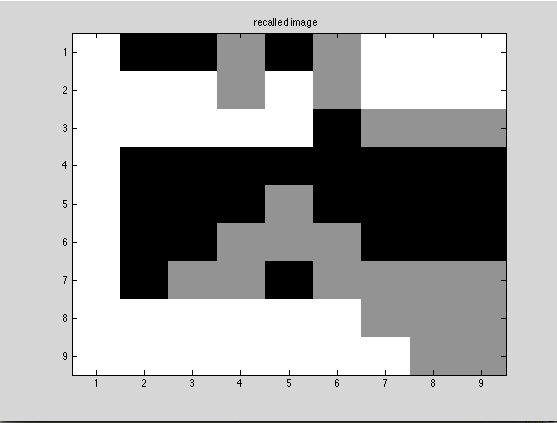
\includegraphics[scale=0.42]{pic2}
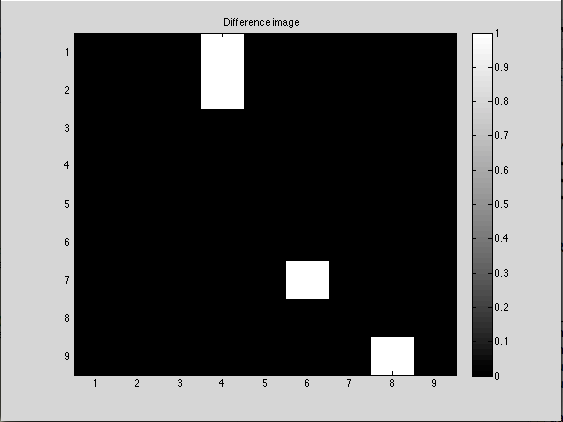
\includegraphics[scale=0.42]{pic3}
\end{center}
\textbf{(Left)} The original classification regions that the LVQ was trained on \textbf{(Righ)} The classification regions that the LVQ outputted \textbf{(bottom) A plot of blocks that were misclassified}\\
\newline
To begin with, the LVQ was trained on a 9x9 matrix, consisting of the numbers 1,2,3. Each number represented a different classification class and this training data is visually represented as the image on the left. One the image on the right and below, you can see that while the LVQ has not perfectly finished learning the training data, with an error rate of 4/81 (4.9 percent), this was deemed acceptable. 
\section*{b)}
\begin{center}
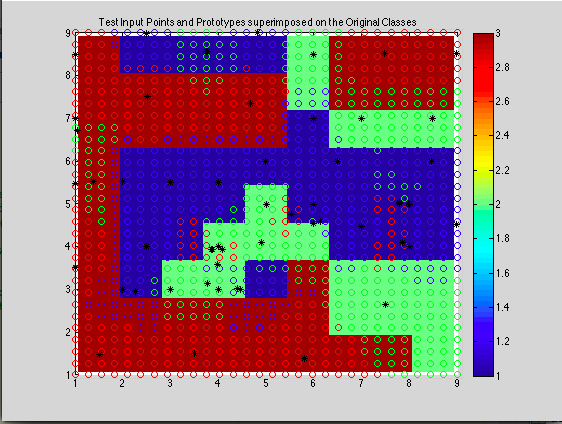
\includegraphics[scale=0.42]{pic4}
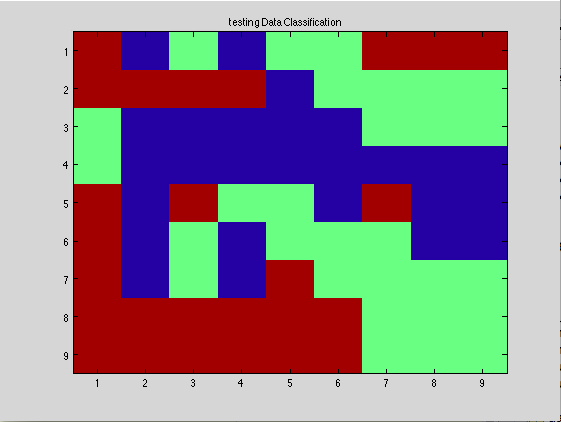
\includegraphics[scale=0.42]{pic5}
\end{center}
\textbf{(Left)} A plot of the Testing Inputs points (circles) and the prototypes (black asterisk) superimposed over the Original classes \textbf{(Right)} Classes based on the testing classes.\\
\newline
After the LVQ has finished training, 900 datapoints were generated in a grid streatching from (1,1) to (9,9). These points were then fed to the LVQ algorithmn which designated the classes as seen in the figure on the left. From this plot, it seems that the LVQ has done a fair job of classifying points as most of the test points are in the correct regions. However the plot on the right illustrates the limitations of the simplistic LVQ algorithmn. In this plot, for every 1x1 block, the containing test points were viewed and the block was painted with the color of the most populous class. But from the plot on the right, we can see the limitations of the LVQ algorithmn. The LVQ algorithmn is not very good at working at these fine boundries. Moreover, there are many protoypes that are completley encompased by other colors. So when you look at the classification done on the test data in terms of most common class, the LVQ does not seem to cut it. An algorithmn such as an SOM or a smarter LVQ such s LVQ2 or3 seems necessary to correctly learn the space.
\newpage
\section*{Question 2.1}
By calling the princomp function on zero meaned inputs, we got the following eigenvalues and eigen vectors:
\[
v_1 = 
\begin{bmatrix}
    0.3996       \\
    -0.1953       \\
    0.6118       \\
    0.6541
\end{bmatrix}
v_2 = 
\begin{bmatrix}
    0.4330       \\
    0.8988       \\
    -0.0479      \\
    0.0487
\end{bmatrix}
v_3 = 
\begin{bmatrix}
     0.7435       \\
    -0.3248       \\
    0.0345       \\
    -0.5835
\end{bmatrix}
v_4 = 
\begin{bmatrix}
    -0.3162       \\
    0.2203       \\
    0.7888      \\
    -0.4789
\end{bmatrix}
\]
With eigenvalues:
$$\lambda_1  =0.2404, \lambda_2 = 0.0277, \lambda_3 = 0.0122, \lambda_4 = 0.0018 $$
And to confirm,
\[
\begin{bmatrix}
    0.3996  &  0.4330  &  0.7435 &  -0.3162 \\
   -0.1953  &  0.8988 &  -0.3248  &  0.2203 \\
    0.6118 &  -0.0479   & 0.0345   & 0.7888 \\
    0.6541  &  0.0487 &  -0.5835  & -0.4789 \\
\end{bmatrix}
\begin{bmatrix}
    0.3996 &  -0.1953 &   0.6118  &  0.6541\\
    0.4330   & 0.8988  & -0.0479   & 0.0487\\
    0.7435  & -0.3248  &  0.0345  & -0.5835\\
   -0.3162 &   0.2203 &   0.7888 &  -0.4789\\
\end{bmatrix}
 = 
 \begin{bmatrix}
    1 &  0 &   0  &  0\\
    0   &1  & 0   & 0\\
    0  & 0  &  1  & 0\\
   0 &   0 &   0 &  1\\
\end{bmatrix}
\]
\newpage
\section*{Question 2.2}
 \begin{table}[htbp] 
\center
\caption{Parameters for GHA}
  \label{tab:NP}
  %\scalebox{0.9}{ % You can scale the size of the table by changing this number
   \scalebox{1.0}{
   \begin{tabular}{p{4cm} p{.05cm} p{8cm}}
\toprule
  \multicolumn{3}{l}{\bf Network parameters} \\
\bottomrule \noalign{\smallskip}
  Topology & & $(4)$ --- $(4)$ \\
  Transfer function & & Identity Transfer Function \\
\toprule
  \multicolumn{3}{l}{\bf Learning parameters} \\
\bottomrule \noalign{\smallskip}
  Initial weights & & drawn from U[-0.1, 0.1] \\
  Learning rate ($\alpha$) & & 0.001\\
  Stopping criteria & &  Mean Absolute Error (see Formula 1) $ \le 0.02 $ OR  learn count (t) $ > 200,000 $\\
  Error measure ($Err_{stop}$)& &  (see Formula 1) \\\toprule
 \multicolumn{3}{l}{\bf Input / output data, representation, scaling} \\
\bottomrule \noalign{\smallskip}
  \# training samples ($N_{tr}$)& & 75 4-D vectors from the Iris Dataset\\
  Scaling of inputs & &  The inputs were transformed to have a mean of zero in each column \\
  Scaling of outputs & &  None \\
%  %\# learn steps performed & & 180,365 (error threshold reached)\\
\toprule
  \multicolumn{3}{l}{\bf Parameters and error measures for performance evaluation} \\
\bottomrule \noalign{\smallskip}
  Error of fit ($Err_{fit}$) & & Formula 1\\
  Final Error of fit for Training Data && 0.1100\\
  \# learn steps performed & & 200,000 (threshold for $Err_{stop}$ reached)\\
  Monitoring frequency ($m$) & & 1,000 learning steps\\

 \bottomrule \noalign{\smallskip}
 
  \end{tabular}
   } % end scalebox
\end{table}
\textbf{Formula 1)}
Mean Absolute Error
$$\frac{1}{75} \sum_{1} ^ K \frac{1}{16} \sum_{i=1}^4 \sum_{j = 1}^4 |A^k_{i,j} - I_{i,j}| $$
Where $A_{i,j}^K$ is the i,j th output of the GHA for input pattern k and I is the identity matrix. The advantage of choosing this metric over others is that it has a very intutive interpretation. The value represents the average difference between an entry of the matrix A and the identiy matrix averaged over all of the training samples. So if the Mean Absolute Error is 0.5, then we know that averaged over all of the training samples, each entry of the matrix is on average, 0.5 from the value of the identity matrix.
\newpage
\textbf{Initial Weight Matrix}\\
The entries weight matrix was generated from a uniform distribution from -0.1 to 0.1. Not suprisingly, it looks nothing like the eigenvectors or the identity matrix.
\[
\begin{bmatrix}
    0.0543 &  -0.0003  & -0.0662 &  -0.0992 \\
   -0.0958 &  -0.0550 &  -0.0823 &   0.0024 \\
    0.0267 &  -0.0604  &  0.0371  &  0.0625 \\
    0.0498 &   0.0521  &  0.0907  &  0.0225 \\
\end{bmatrix}
\]
\textbf{Weight Matrix after GHA Learning}
\[
\begin{bmatrix}
    0.3995 &   0.4277 &   0.7426&    -0.2942 \\
   -0.1896 &   0.9012  & -0.3263 &   0.0564 \\
    0.6117 &  -0.0488  &  0.0361&   -0.0018 \\
    0.6560  &  0.0508 &  -0.5828 &   0.2155 \\
\end{bmatrix}
\]
\textbf{Absolute Value of the Difference between Desired and GHA Learning}
\[
\left | \begin{bmatrix}
    0.3996  &  0.4330  &  0.7435 &  -0.3162 \\
   -0.1953  &  0.8988 &  -0.3248  &  0.2203 \\
    0.6118 &  -0.0479   & 0.0345   & 0.7888 \\
    0.6541  &  0.0487 &  -0.5835  & -0.4789 \\
\end{bmatrix} 
-
\begin{bmatrix}
    0.3995 &   0.4277 &   0.7426&    -0.2942 \\
   -0.1896 &   0.9012  & -0.3263 &   0.0564 \\
    0.6117 &  -0.0488  &  0.0361&   -0.0018 \\
    0.6560  &  0.0508 &  -0.5828 &   0.2155 \\
\end{bmatrix}
\right |
\]
$$ 
=
\begin{bmatrix}
    0.0001 &   0.0053 &   0.0009&    0.022 \\
   0.0057 &   0.0024  & 0.0015&   0.1639 \\
    0.0001 &  -0.0009  &  0.0016&   0.7906 \\
    0.0019  &  0.0021 &  0.0007 &   0.6944 \\
\end{bmatrix}
$$
After an extremely lengthy 200,000 learning steps, the GHA has presented a matrix of eigenvectors that at first seems nearly identical. But if you observe the absolute value of the difference bteween the desired and the GHA learning, you can see that the 4th column (4th eigenvector) has not still not been able to make the 4th eigenvector converge to the correct value. This is because with each progressive eigenvector, the algorithmn takes longer and longer to run. So the 1st eigenvector will be the first to converge. Then the second, and lastly the 4th.\\
\newline

\newpage
\textbf{Learning History}
\begin{center}
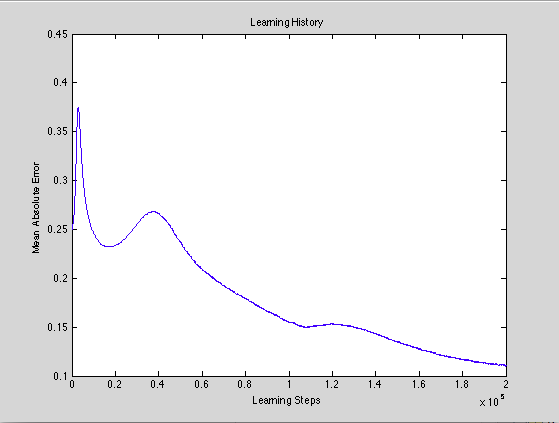
\includegraphics[scale=0.7]{pic6.png}
\end{center}
For the Learning History, instead of an L2 norm, the error metric that was chosen was Mean Absolute Error. As mentioned earlier, the advantage of choosing this metric over others is that it has a very intutive interpretation. The value represents the average difference between an entry of the matrix A and the identiy matrix averaged over all of the training samples. So we know that when the weights were initialized, they each entry of the matrix was on average 0.25 from the idenity matrix. But by the end, that value has managed to decrease to 0.11. At first this may seem quite bad. But if you recall that the GHA algorithmn finds the most important 1st principal componant first, then the second most important, 2nd principal componant second, the vast majority of the error is coming from the least important 4th principal componant. And the 4th componant has a tiny 0.0018 eigenvalue compared to the 1st componant which has 0.2404. A difference of 134 times! So in summary, it seems fair to say that barring the not too important 4th princiapl componant, the GHA has done a good job learning the matrix. However, espeically with matricies that are this small, it is by far quicker to run princomp or a comparable function rather than to run a GHA. For the GHA to become useful, perhaps the dimensionality of the data needs to be increased many fold--to the point where it becomes expensive to do large matrix operations while the cost of running GHA doesnt increase as much.
\end{document}


